\section{Numerical projection and generative information}\label{sec:numerical}
Fix a source $m_0$. Let $\Hist(m_0)$ be the set of histories from $m_0$. Three projections are in play:
\[
\Hist(m_0)\xrightarrow{\ \pi_1\ }\mathrm{Cls}(m_0)\xrightarrow{\ \pi_2\ }\mathrm{Cont}(m_0)\xrightarrow{\ \pi_3\ }\mathrm{End}(m_0)\subseteq\Z,
\]
\[
h\mapsto[h]\mapsto c(h)\mapsto m_0\prod_NR(N)^{c_N}=\Endp(h).
\]
Here $\mathrm{Cls}(m_0)$ is the set of swap classes (all words in a class have the same content, since legal swaps are transpositions) and $\mathrm{Cont}(m_0)$ the set of contents of admissible histories, and $\mathrm{End}(m_0)=\{\Endp(h)\}$ the set of reachable endpoints; the codomain of $\pi_3$ is $\mathrm{End}(m_0)$, not all of $\Z$, so that $\pi_1,\pi_2,\pi_3$ are surjections. For a finite alphabet $A$ write $\mathrm{Cont}_A(m_0)\subseteq\mathrm{Cont}(m_0)$ for the admissible contents supported on $A$, $\mathrm{End}_A(m_0)$ for the endpoints of histories over $A$, and $\pi_{3,A}:\mathrm{Cont}_A(m_0)\to\mathrm{End}_A(m_0)$ for the restriction of $\pi_3$; the matrix $V_A$ acts on $\Z^A$ and so only on contents supported on $A$.

\subsection{Cited ingredients}
\begin{theorem}[kernel condition; \Src{II}{thm:kernel}]\label{thm:kernel-cited}
Let $A$ be a finite alphabet, $\mathcal P$ the primes dividing some $N$ or $N+1$, $N\in A$, and $V_A=(\Delta_p(N))_{p\in\mathcal P,N\in A}$ with $\Delta_p(N)=2v_p(N+1)-v_p(N)$. Two histories over $A$ from the same source have the same endpoint iff $V_A(c-c')=0$.
\end{theorem}
\begin{theorem}[faithfulness; \Src{II}{thm:faith}]\label{thm:faith-cited}
For a fixed source the fibre sequence $F(h)$ determines the history $h$. A legal swap changes exactly one entry of $F(h)$.
\end{theorem}
\begin{theorem}[classification for $\{2,3,14\}$; \Src{II}{thm:2314}]\label{thm:2314-cited}
The number $\nu(m)$ of swap classes of $\{2,3,14\}$ at the source $m$ is $0$ if neither $14$ nor $21$ divides $m$, $2$ if $14\mid m$ and $\gcd(m/14,6)=1$, and $1$ otherwise.
\end{theorem}

\subsection{The proposition}
\begin{proposition}[\SIV{1}: endpoint projection and retained information]\label{prop:P1}\status{new, proved}
Let $m_0\ge1$.
\begin{enumerate}[label=(\alph*),itemsep=1pt]
\item \emph{Factorization.} The maps $\pi_1,\pi_2,\pi_3$ are well defined and $\Endp=\pi_3\pi_2\pi_1$. Thus the endpoint is a function of the content, and of the swap class, of the history; and a numerical invariant of the endpoint is a function of $(m_0,\text{content})$.
\item \emph{What the endpoint retains.} For histories over a common alphabet $A$ the endpoint determines exactly the vector $V_Ac=(v_p(t)-v_p(m_0))_{p\in\mathcal P}$, and conversely this vector determines the endpoint. The fibre of $\pi_{3,A}$ over a reachable endpoint $t=\Endp(h)$ with $h$ over $A$ is $\pi_{3,A}^{-1}(t)=\mathrm{Cont}_A(m_0)\cap\bigl(c(h)+\ker_{\Z}V_A\bigr)$: the coset must be intersected with the set of \emph{admissible} contents from $m_0$ supported on $A$, not merely with $\N^A$. (Histories using letters outside $A$ and ending at $t$ are in the fibre of $\pi_3$ but not of $\pi_{3,A}$; they are compared by enlarging $A$.) Example: $m_0=1$, $A=\{1,2,3\}$, $c=(7,0,0)$ and $c'=(0,2,4)$ have $R(1)^7=R(2)^2R(3)^4=16384$, so $c-c'\in\ker_\Z V_A$ and $c'\in\N^A$, yet $c'\notin\mathrm{Cont}_A(1)$ because neither label $2$ nor label $3$ can be applied first.
\item \emph{Each projection is non-injective.} (i) $\pi_3$: at $m_0=32$ the histories $(2,2,2,2)$ and $(1,8,8)$ are admissible with the same endpoint $13122$ and different content and length. (ii) $\pi_2$: at $m_0=14$ the contents of $(14,3,2)$ and $(2,3,14)$ coincide, both end at $5400$, but they lie in different swap classes. (iii) $\pi_1$: from $m_0=1$ the two histories $(1,2,1),(1,1,2)$ to $72$ lie in one class.
\item \emph{Invariants.} Functions of $(m_0,\Endp(h))$ factor through $\pi_3\pi_2\pi_1$ (this includes, for fixed $m_0$, the number $H(m_0,t)$ of histories from $m_0$ to $t$, which depends only on $t$); the length $r$ of $h$, the content and the swap class do not factor through $\pi_3$ on any set of sources containing the witnesses in (c). The number of histories to $t$ is a function of $t$ but does \emph{not} factor through the occurrence set $D(t)$ (\cref{prop:P5}).
\end{enumerate}
\end{proposition}
\begin{proof}
(a) A legal swap exchanges two adjacent letters, so the content is invariant; hence $\pi_2$ is defined on classes. The product formula $\Endp(h)=m_0\prod R(N_i)$ gives $\pi_3$. (b) is \cref{thm:kernel-cited} together with the identity $v_p(\Endp(h))-v_p(m_0)=\sum_N c_N\Delta_p(N)=(V_Ac)_p$, which follows from $v_p(R(N))=2v_p(N+1)-v_p(N)$. For the fibre: a content $c'\in\mathrm{Cont}_A(m_0)$ has the endpoint $t$ iff $V_A(c'-c)=0$, i.e.\ iff $c'\in c+\ker_\Z V_A$; the example has $V_A(c-c')=0$ by $R(1)^7=4^7=16384=(9/2)^2\cdot(16/3)^4$, and $c'$ is inadmissible from $1$ since admissibility of a first letter $N$ requires $N\mid m_0=1$. (c)(i): $T_2$ applied to $32,144,648,2916$ (all even) gives $144,648,2916,13122$; and $32\to128\to1296\to13122$ by $T_1,T_8,T_8$ with $8\mid128$ and $8\mid1296$. Lengths are $4$ and $3$. (ii): $14\to225\to1200\to5400$ by $T_{14},T_3,T_2$ with $3\mid225$, $2\mid1200$, and $14\to63\to336\to5400$ by $T_2,T_3,T_{14}$ with $3\mid63$, $14\mid336$. By \cref{thm:2314-cited} with $m=14$ ($14\mid14$, $\gcd(1,6)=1$) there are two classes; the only admissible arrangements are these two. (iii): $72=1\cdot4\cdot\tfrac92\cdot4$ and the two words differ by one legal adjacent transposition. (d) The first sentence follows from (a) and \cref{lem:factor}; the non-factorization of $r$, content and class through $\pi_3$ is the witnesses of (c). For the last sentence: the count $H(m_0,t)$ is by definition constant on the fibres of $\pi_3$, and its failure to factor through $D(t)$ is the witness pairs of \cref{prop:P5}.
\end{proof}
\begin{remark}
\cref{prop:P1}(b) is the precise sense in which the endpoint is a \emph{valuation-displacement}: it forgets how that displacement was composed from letters. The identity $\sum_Nc_N\Delta_p(N)=(V_Ac)_p$ is the same arithmetic that organises the gain--loss accounting of \Src{III}{thm:B2T3}.
\end{remark}

\noindent\Cref{fig:endpoint} shows endpoint projection and its fibres.

\begin{figure}[t]\centering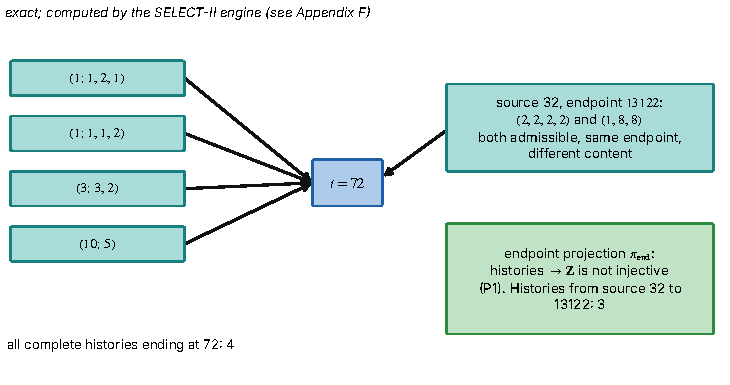
\includegraphics[width=\linewidth]{fig03_endpoint_fibres.pdf}
\caption{\textbf{Endpoint projection and its fibres} ($\pi_3$ of \cref{prop:P1}). Left: the four complete histories that end at $72$, from sources $1,1,3,10$. Right: two histories from source $32$ with the same endpoint and different content. \emph{Exact; computed by the history engine (Appendix~\ref{app:finite}).}}\label{fig:endpoint}\end{figure}

\noindent\Cref{fig:anc72} shows four histories reaching $72$ and their structural records.

\begin{figure}[t]\centering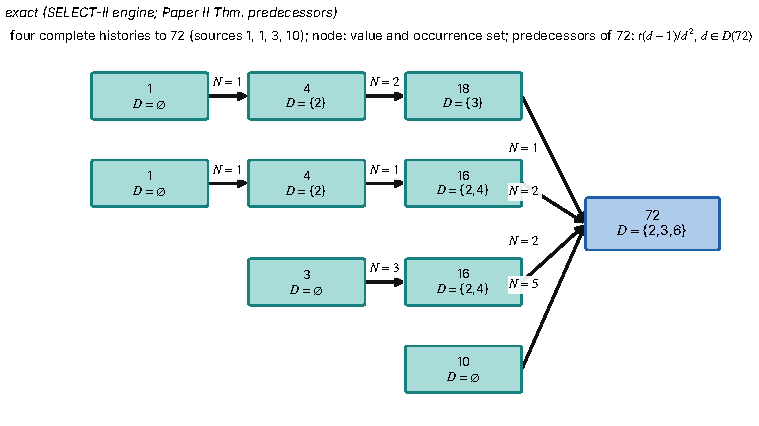
\includegraphics[width=\linewidth]{fig04_ancestry_72.pdf}
\caption{\textbf{Four histories reaching $72$ and their structural records.} Each node shows an integer and its occurrence set $D$; arrows are SELECT-II steps labelled by $N$. The four paths have different fibre sequences $F(h)$, although they share the endpoint $72$ and the same terminal data $D(72)=\{2,3,6\}$ (\Src{II}{thm:predecessors}, \Src{II}{thm:faith}). \emph{Exact.}}\label{fig:anc72}\end{figure}

\noindent\Cref{fig:kernel} shows same endpoint, different label content.

\begin{figure}[t]\centering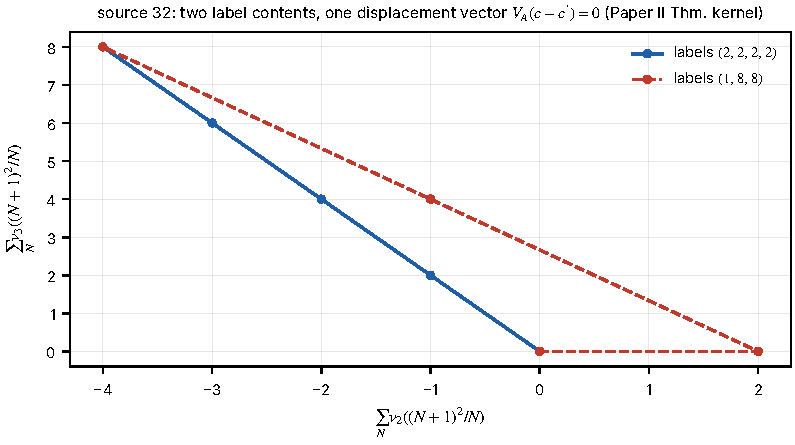
\includegraphics[width=0.85\linewidth]{fig05_kernel_ambiguity.pdf}
\caption{\textbf{Same endpoint, different label content.} Cumulative displacement of $(v_2,v_3)$ of the running value for the label words $(2,2,2,2)$ and $(1,8,8)$ from source $32$: both paths end at $V_A c=V_Ac'$ (\cref{thm:kernel-cited}). \emph{Exact.}}\label{fig:kernel}\end{figure}
